\chapter{Introduction} % Main chapter title
\label{chp:introduction} 

%\todo{numbers!}

Modern online companies make broadly use of cloud computing infrastructures for 
carrying their business.
Among the public cloud providers, the most popular and technologically advanced 
are Amazon Web Services (AWS), Microsoft Azure (Azure), and Google Cloud 
Platform (GCP)~\citep{flexera_report}.
To have a glance about the turnover, the second quarter of 2020 showed a growth 
of $62$\% of Azure respect the same period in the 
previous year, with investments of $79.9$M USD, $78$M 
USD, and $76.7$M USD from Verizon, MSI Computer, and LG Electronics, 
respectively~\citep{azure_business}.
We can observer similar figures in Amazon AWS services, that declared $1$M of 
active users in 2020, with $18$M USD invested by Netflix in the same 
year~\citep{aws_business}.
Still in 2020, $786$ tech companies choose GCP for their 
businesses~\citep{google_business}.

The widespread of cloud computing technologies arose the attention of security
experts concerning the protections of third part 
infrastructures~\citep{ryan2011cloud,sun2014data}.
Check Point and McAffe surveyed the possible threats that could target
cloud services~\citep{checkpoint_cloud,mcaffee_cloud}.
Such problems reveal to be even more critical when considering that a huge part 
of could infrastructures (\ie the host machines) are out of the companies 
control.
In this scenario, leaving part of the control to the could provider means 
trusting that a list of issues are already addressed at vendor side (\eg Azure 
or AWS).
The source of risk are various, for instance, the cloud provider might suffer 
of insider threats, \eg a GCP employ, with access to physical machines, could 
record the network traffic, access to the user's data, or tamper with the 
virtual machines (VM) themselves~\citep{insider_threat}.
Even if we assume having a trusted provider, recent works showed that two VMs, 
sharing the same host, can exchange information solely relying on the CPU 
cache~\citep{maurice2017hello}. This means that that a VM can carry attacks 
toward other VMs on the same host.

Having a cloud infrastructure introduces security risks also for the final 
user. In fact, a remote client (\eg a smartphone) has no guarantees to 
communicate with the the correct software in the remote 
VM~\citep{beekman2016attestation}, \eg a malicious hypervisor may manipulate 
the physical pages and force a VM to load non-intended 
content~\citep{10.1145/3292006.3300022}.
Another source of insecurity comes from the stored data: passwords and critical 
information are saved in non-volatile devices (\ie hard-drives) that are under 
control of the cloud provider as well, thus inevitably leading to integrity and 
confidentiality issues.
In this scenario, classic cryptography solutions fail since the whole system 
might be compromised, \ie the cloud provider may control the cryptographic keys.
Even though one could adopt mitigation to obtain reasonable guarantees, such 
as the intended software is properly loaded (\ie using TPM to protect 
the boot phase -- \cite{tpm-isoosi}), the underline system is secure (\ie 
through strict contracts or dedicated hosts -- \cite{aws_dedicated_host}), and
the data are sealed properly (\ie using modern crptographic 
schemes -- \cite{gentry2009fully}).
These solutions are rarely used in practice because either expensive or non 
scalalbe. The former requires dedicated hosts that are far more expensive than 
standard solutions, moreover TPMs are not usually provided by cloud vendors. 
The latter involves heavy cryptographic schemes that are too slow for 
being vastly used in daily business~\citep{10.1145/2046660.2046682}.
%
In addition to all the aforementioned problems, one should also consider 
classic exploitation techniques that may alter the logic of a piece of software 
by targeting the perimeter of a system.
In this scenario, an adversary may target error-prone services exposed over the 
Internet, and take control of 
machine~\citep{van2012memory,10.1145/2810103.2813646}.
Finally infecting the system.

%\todo{possible solution: TEE. Give intuitive definition.}
For tackling the aforementioned challenges, a promises direction is 
represented by Trusted Execution Environments (TEE).
Intuitively, TEEs are sub-systems, whose functioning remembers virtual 
machines, that use hardware features to isolate their content against untrusted 
environments.
%\todo{Definition of TEE and usage. Properties, memory isolation, and remote 
%attestation.}
%\todo{History of TEEs, first definition, standard used, etc. During the 
%	description, stay "high level" and recall properties and differences. This 
%	should give a context.} 
The TEEs are controlled by the main CPU, that represents the primary source of 
trust, and enable a user to define \emph{trusted memory regions} in the main 
memory (RAM)~\citep{Sabt2015TrustedEE}.
Historically, the first formal definition of TEE has been proposed by OMTP, 
whose design was mainly focused on mobile platforms~\citep{omtp}.
OMTP defines a list of properties that a TEE should fulfill, among them, this 
thesis will trait the \emph{memory isolation} and the \emph{remote attestation}.
The main purpose of the \emph{memory isolation} is to shield code and data such 
that even a compromised machine cannot alter its integrity (and 
confidentiality).
In particular, the \emph{memory isolation} must prevent tampering from any 
sources at any privilege level, \eg it must avoid writing and reading 
operations from the operating system, the SMM code~\citep{yao2009system}, and 
DMA transfers~\citep{coke1998implementing}.
The \emph{remote attestation} guarantees that a third party (\eg a smartphone) 
can verify the integrity of a remote memory region (\eg on a server).
This ensures that a client is communicating with the intended portion of code 
and machine (usually represented by the CPU).
The combination of \emph{memory isolation} and \emph{remote attestation} leads 
to a new range of properties in the cloud environments, \ie a company 
can use the \emph{memory isolation} to protect critical piece of 
software and date from insiders, a compromised host, or even other VMs sharing 
the same resources.
In addition, the \emph{remote attestation} allows the establishment of 
end-to-end secure channels without the support of the OS, thus mitigating 
network analysis.
Finally, the TEEs can use attestation to seal data on non-volatile storage (\ie 
encrypt and decrypt) such that nobody but the original \emph{trusted region} 
can retrieve the content. 
Even though TEEs seem sharing similarities with TPM technologies, they differ 
from many perspectives.
For instance, TMPs require an external hardware (\ie the TPM module), while 
TEEs are embedded in the main CPU.
Moreover, TPMs do not provide memory isolation, can only store limited 
cryptographic material (\eg keys), and expose a limited number functionalities 
(\eg random number generation or cryptographic primitives).
On the contrary, TEEs are meant to contain general purpose software that might 
interact with the peripherals.
In chapter~\ref{chp:background}, we detail the TEE background.

From the first OMTP definition, many vendors proposed their own TEE technology 
on the market.
In 2012, Intel proposed  Trusted Execution Technology 
(TXT)~\citep{greene2012intel} to measure the software integrity.
In 2014, ARM introduced the TrustZone technology in new lines of CPU and 
controllers~\citep{arm-trustzone}. 
%TrustZone devices can bootstrap two parallel OSs: one called \emph{enriched} 
%OS, that should handle all the normal operations; and a second one called 
%\emph{trusted} OS, with the duty to containing critical applications.
More recently, AMD proposed Secure Encrypted Virtualization 
(SEV)~\citep{amdsev}, that shields whole VMs from their host, and 
Apple proposed a similar technology for their smartphones \citep{apple-enclave}.
Among the various technologies, one particularly attracted the attention of the 
cloud market: Intel Software Guard eXtensions (SGX).
Intel SGX was announced in 2013~\citep{rozas2013intel} and is currently adopted 
by many cloud providers, such as Azure~\citep{azure}, 
GCP~\citep{challita2018precise}, IBM~\citep{IBM}, and 
Alibaba~\citep{alibabasgx}.
This technology provides either a strong \emph{memory isolation} and a reliable 
\emph{remote attestation} that stand at the base of many businesses, such as 
Signal~\citep{signal}.
Due to the important growth of SGX in the recent years, and considering its 
adoption in the cloud computing market, this thesis will consider SGX as main 
TEE technology.

\section{SGX Overview}

Describe Figure~\ref{fig:sgx-architecture} and broadly .
In Section~\ref{sec:software-guard-extension}, we discuss the SGX internals.

\begin{figure}[t]
	\centering
	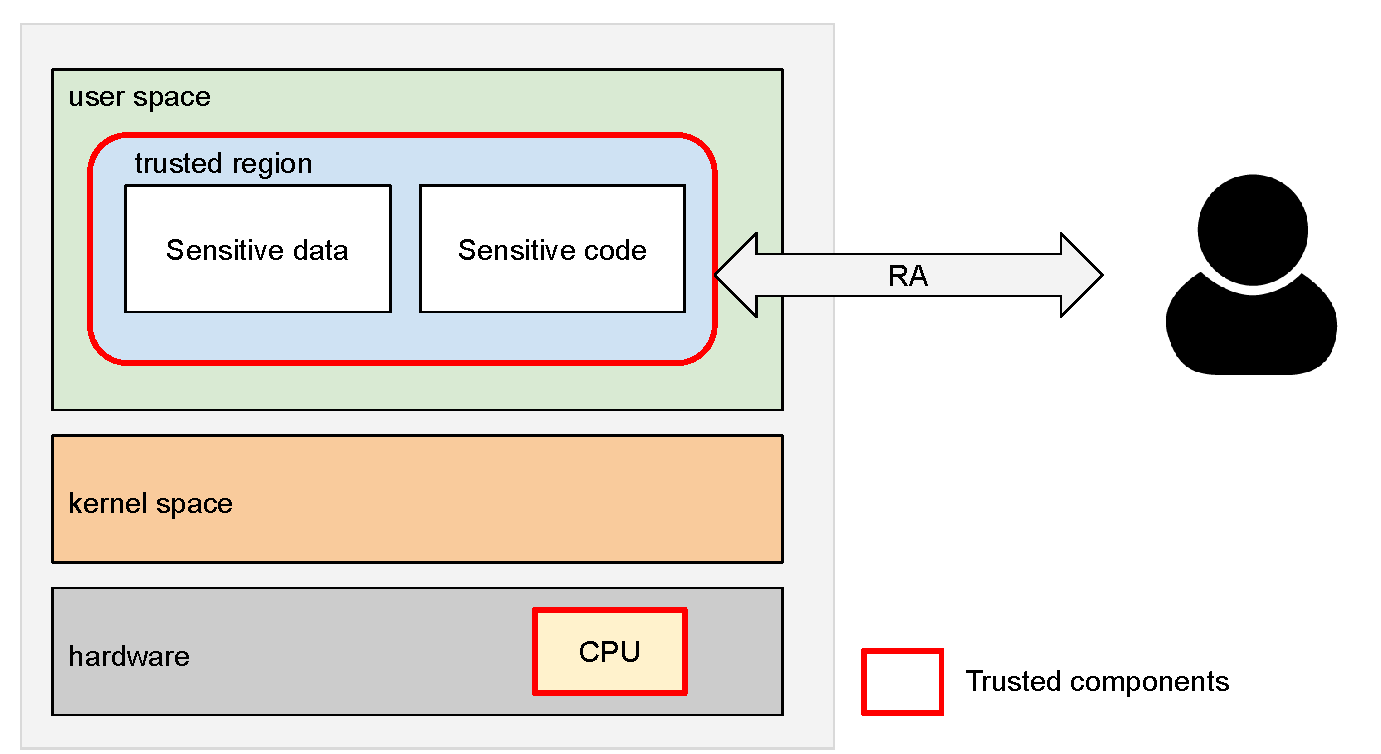
\includegraphics[width=0.5\textwidth]{fig_c1/sgx-architecture.pdf}
	\caption[SGX architecture.]{Simplified SGX architecture.}
	\label{fig:sgx-architecture}
\end{figure}

\section{Thesis Contribution}

\todo{Motivations from Figure~\ref{fig:mind-map}, carry my reasoning and, at 
	each point state explicitly what's the problem.}
\todo{Define 4 areas: (1) Anti-tampering (find a better name), (2) New threats, 
	(3) Runtime RA, (4) Memory forensic. These are taken from the mind-map. For 
	each class, state the problem clearly and list the contribution. Do it in 
	separate subsections. My contribution in Figure~\ref{fig:contribution}.}

\todo{State the \emph{thesis} of the thesis, and the "test" to falsify the 
	thesis.}
My thesis argues that Trusted Execution Environments (TEE), such as SGX, are 
powerful tools that isolate portion of code against strong adversaries (\ie the 
OS itself).
However, TEEs are not the silver-bullet of cyber security and they suffer of 
limitations in terms of scalability and security.

\textbf{MY THESIS OBJECTIVE:}
I argue that we can further extend the TEE properties by carefully choosing 
smarter software design without the need of changing the TEE modules (and thus 
changing the hardware).
Throughout the dissertation, I first investigate the TEE limitations, 
then, I will propose relative solutions.
\todo{I have to discuss every point carefully, this is just a memory for me.}

\todo{Wrap up the limitations from the previous point, and describe the 
	contribution of the thesis in Figure~\ref{fig:contribution}.}

Split the contribution in four sections:

Overall, my study covers five TEE aspect:
\begin{itemize}
	\item \todo{Scalability untrusted code protection} First, I will face a 
	scalability issues that affect many modern	TEE technologies 
	(Section~\ref{sec:contribution1}).
	
	\item \todo{New threats} At this point, I covered static and runtime 
	protection for the untrusted code, now I will investigate new type of 
	threats for the \emph{enclaves} themselves 	
	(Section~\ref{sec:contribution2}).
	
	\item \todo{New defenses} Then. I will extend remote attestation for 
	runtime properties (Section~\ref{sec:contribution3}).
	
	\item \todo{Forensic analysis} Finally, I will investigate the new 
	challenges introduced by TEE technologies in terms of memory-forensic 
	analysis (Section~\ref{sec:contribution4}).
\end{itemize}

\textcolor{red}{\hrule}
\vspace{0.5cm}

\begin{figure}[t]
	\centering
	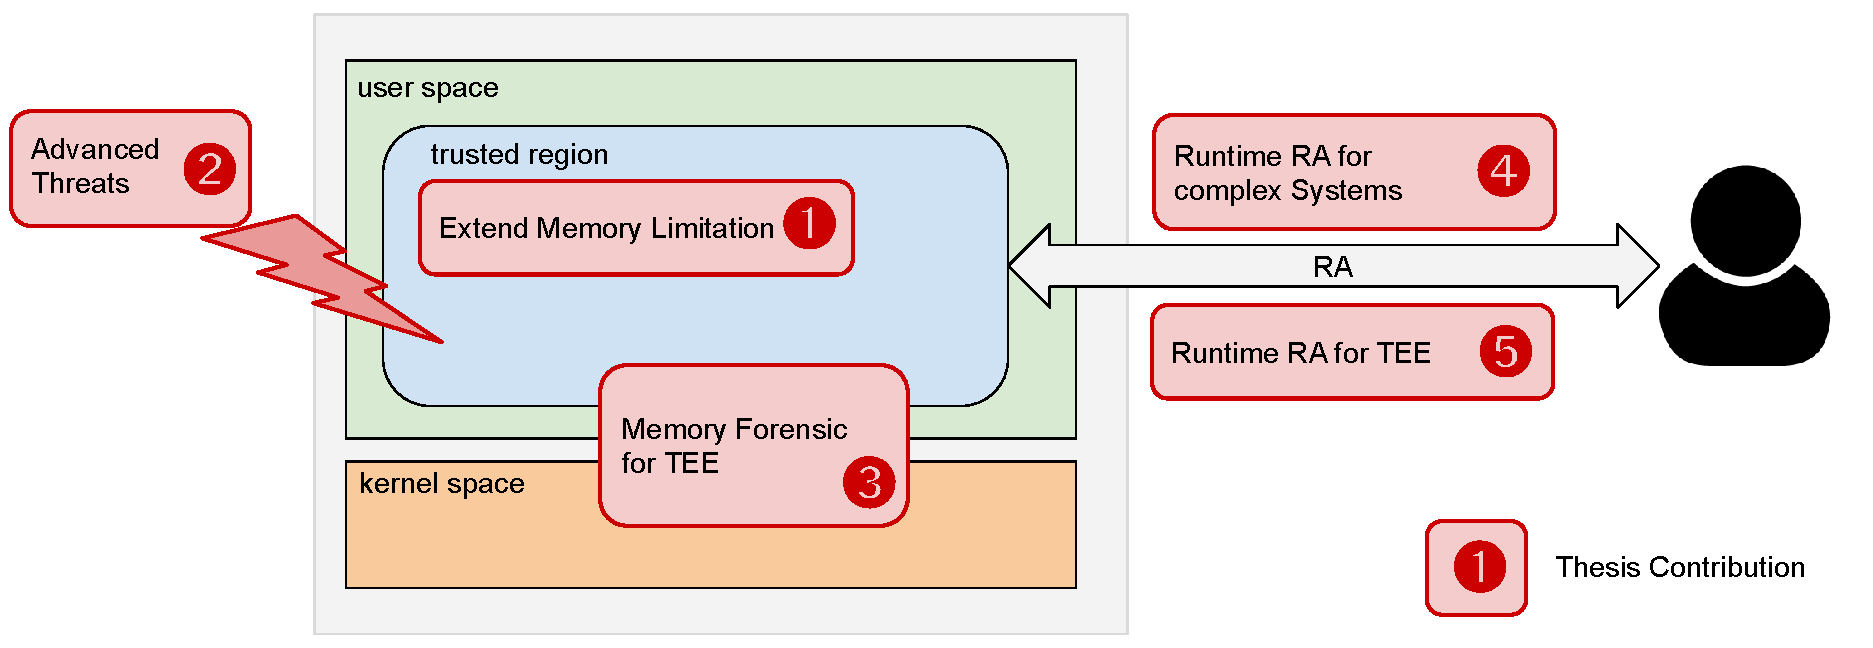
\includegraphics[width=0.7\textwidth]{fig_c1/contribution.pdf}
	\caption[Thesis contribution.]{Thesis contribution.}
	\label{fig:contribution}
\end{figure}

\begin{figure}[t]
	\centering
	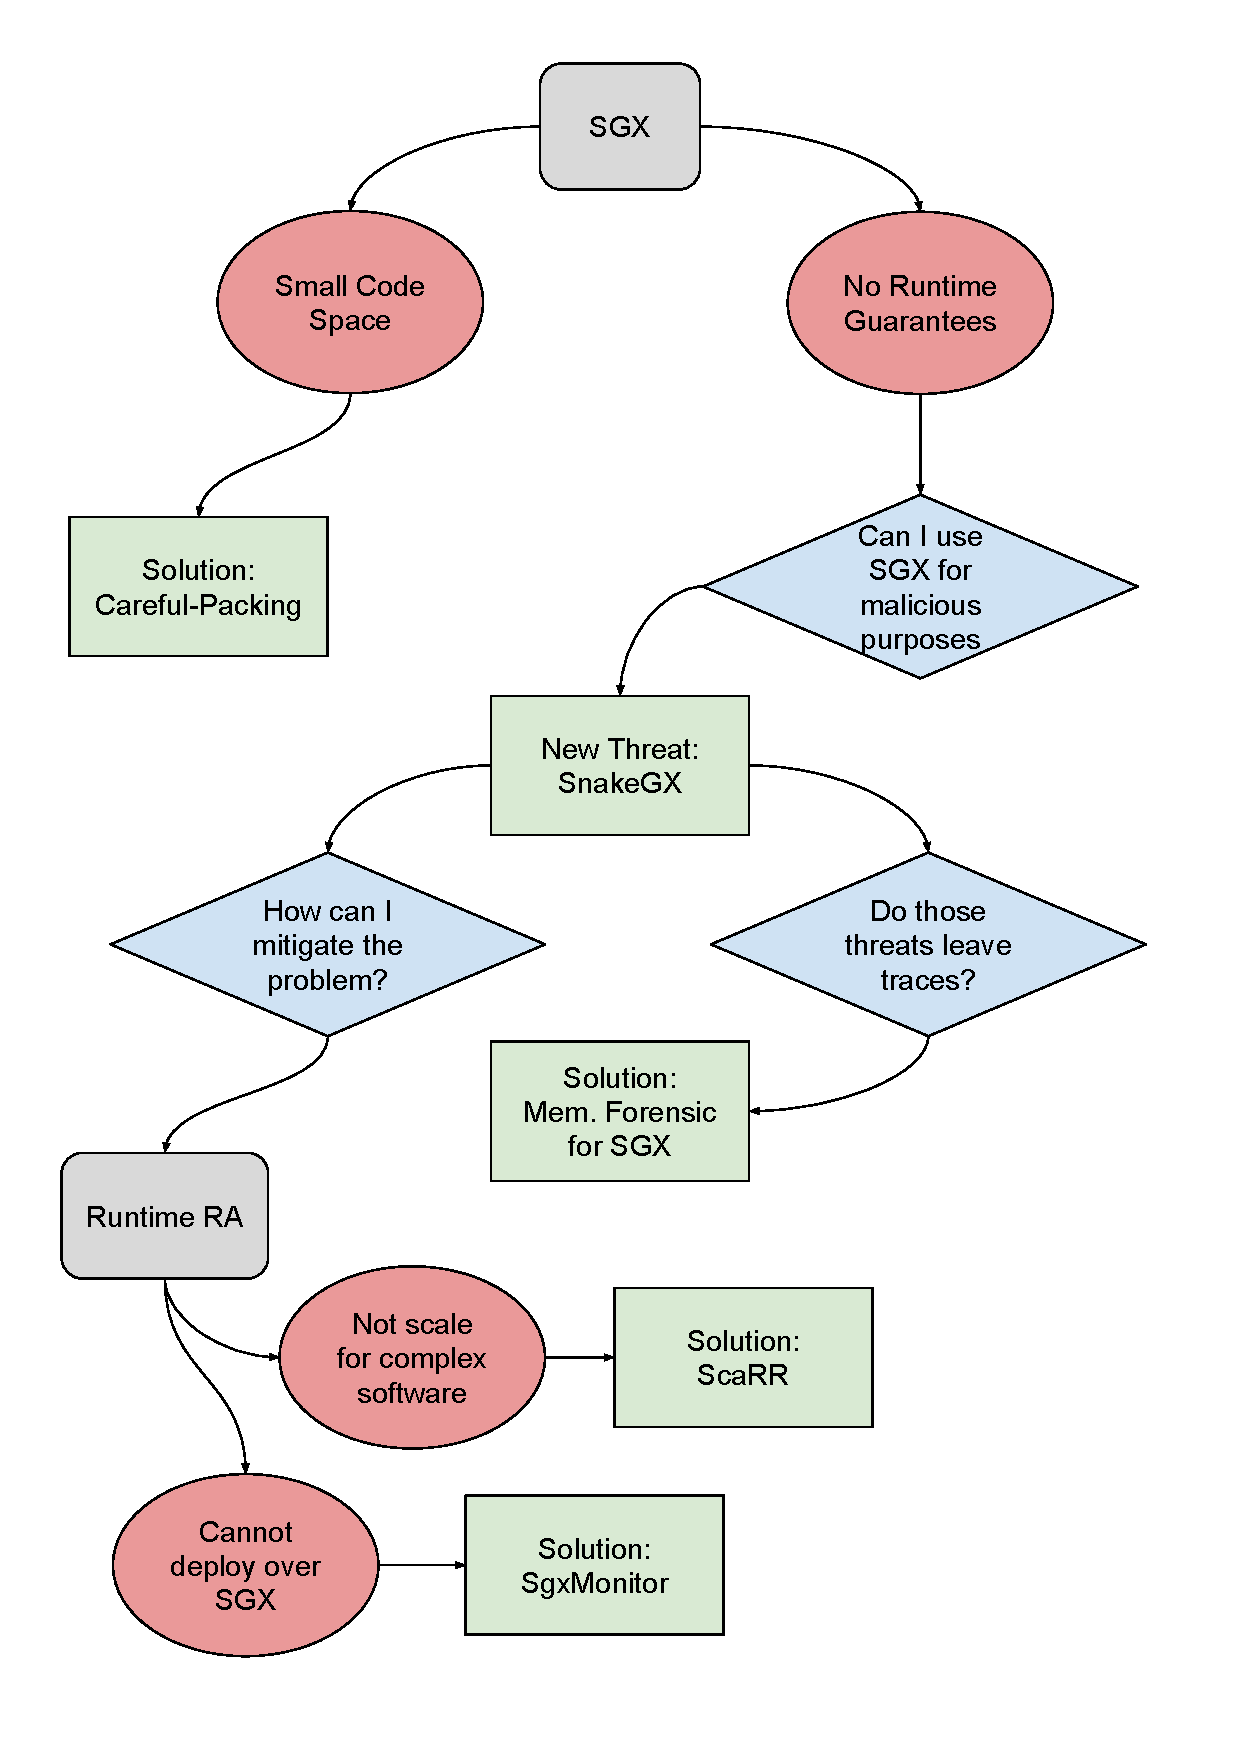
\includegraphics[width=\textwidth]{fig_c1/mind-map.pdf}
	\caption[Mind-map.]{Mind-map (TO REMOVE LATER).}
	\label{fig:mind-map}
\end{figure}


\section{TO-CHANGE Contribution for Software Integrity Limitation}
\label{sec:contribution1}

Then addressed in Chapter~\ref{chp:static-protection}.

\section{TO-CHANGE Contribution for New Threats}
\label{sec:contribution2}

Then addressed in (Chapter~\ref{chp:advanced-threats}).

\section{TO-CHANGE Contribution for Remote Attestation}
\label{sec:contribution3}

Then addressed in Chapter~\ref{chp:runtime-protection-untrusted} and
Chapter~\ref{chp:runtime-protection-trusted}.

\section{TO-CHANGE Contribution for Memory Forensic}
\label{sec:contribution4}

Then addressed in Chapter~\ref{chp:forensic}.

